\chapter{Aufgabe}
\section*{a}
\subsection*{i}
Siehe Abbildung \ref{fig:graphLCOM}

\begin{figure}[h!]
	\centering
	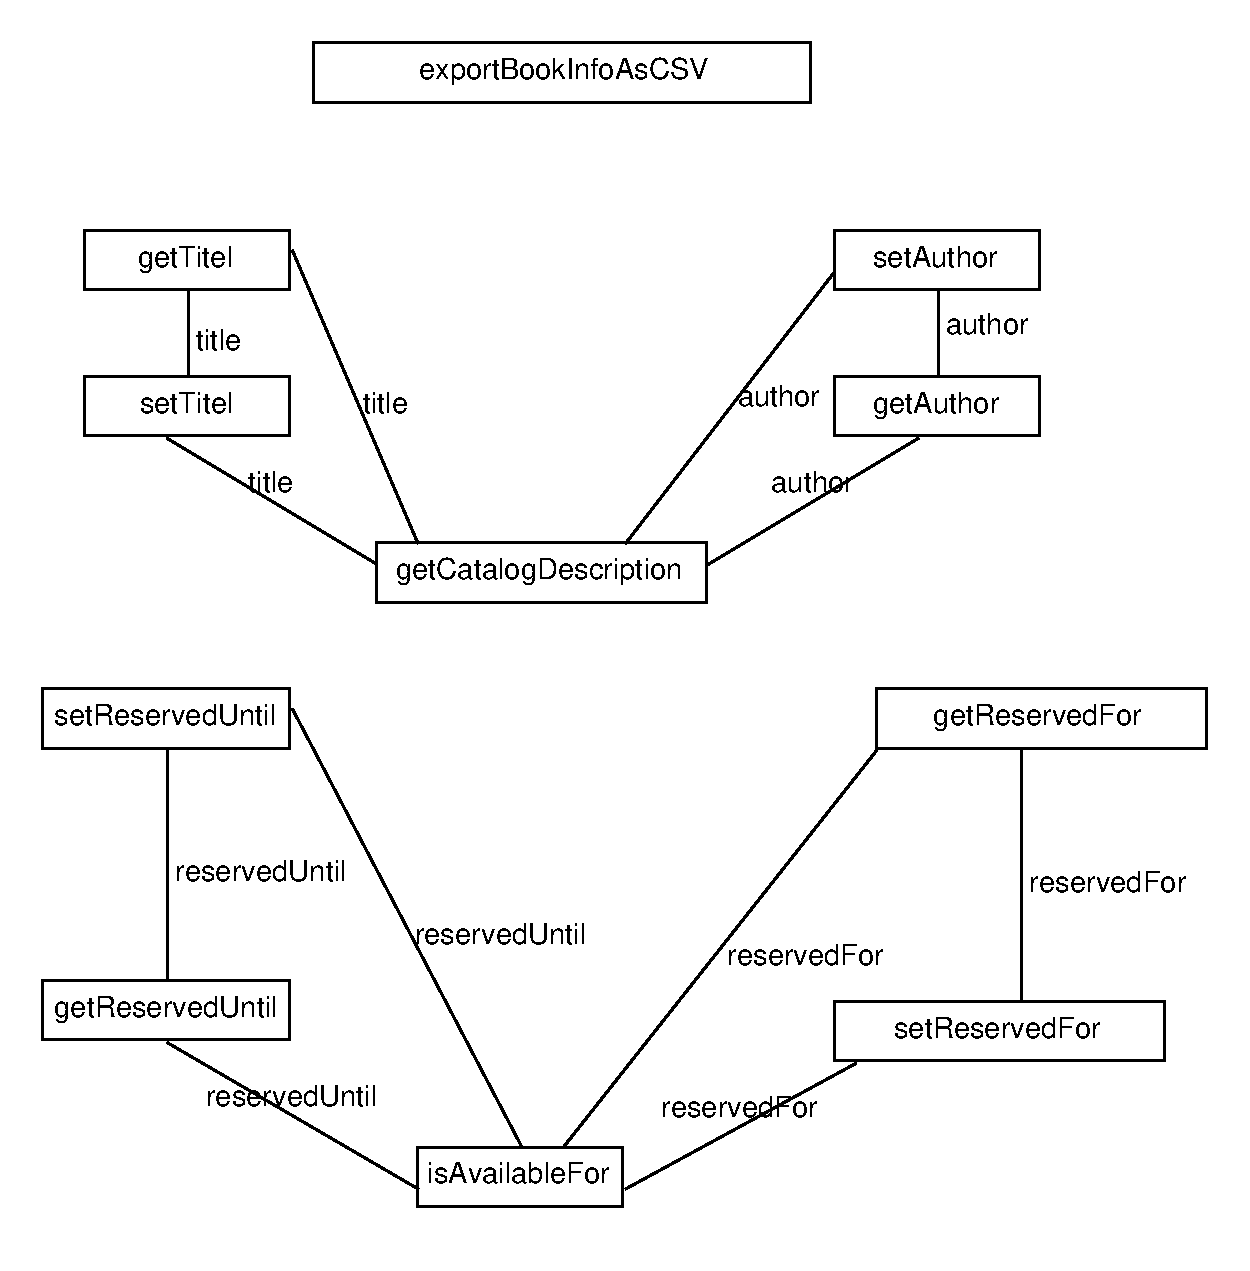
\includegraphics[width=0.8\textwidth, clip]{images/graphLCOM.pdf}
	\caption{Zusammenhangsgraph der Klasse Book für das  LCOM Verfahren. }
	\label{fig:graphLCOM}
\end{figure}
\subsection*{ii}
\textbf{LCOM = 3 von 11}



\section*{b}
Bei erstem Betrachten der Implementation erschien deren Kohäsion nicht optimal zu sein. Drei nicht zusammenfallende Verantwortungen sind alle in einer Klasse enthalten, die noch dazu ein sehr allgemeines Konzept beschreibt, was eine hohe Kohäsion sehr wünschenswert machen würde.\\
Der berechnete Wert spiegelt dies gut wieder, da er mit 3 auf jeden Fall nicht optimal ist. Angesichts der hohen Methodenanzahl in der Klasse hätte er aber dem Empfinden nach noch höher ausfallen können.
Die Verantwortungen der Klasse \texttt{Book} sind:
\begin{enumerate}
	\item Verwaltung der Daten eines einzelnen Buches
	\item Verwaltung der Daten Bezüglich der Ausleihe eines einzelnen Buches
	\item Exportieren der Daten eines einzelnen Buches als csv-Datei
\end{enumerate}
 Der ermittelte \textbf{LCOM}- Wert deckt sich also hier genau mit der Anzahl der Verantwortungen der Klasse. Die Einteilung Anzahl der Responsibilities = LCOM-Ergebnis ist sicherlich oft zutreffend, bei sehr schlechtem Code muss sie aber auch nicht zwangsläufig zutreffen. Mehrere Verantwortungen können sich durchaus überschneiden (sollten es aber generell nicht)
 oder die Methoden einzelner Verantwortungen können auch in keinerlei Bezug stehen (ebenfalls zu vermeiden).
 
 
\section*{c}
\lstset{language=Java,
	showspaces=false,
	showtabs=false,
	breaklines=true,
	showstringspaces=false,
	breakatwhitespace=true,
}


\definecolor{dkgreen}{rgb}{0,0.6,0}
\definecolor{gray}{rgb}{0.5,0.5,0.5}
\definecolor{mauve}{rgb}{0.58,0,0.82}

\lstset{	
	frame=tb,
	language=Java,
	aboveskip=3mm,
	belowskip=3mm,
	showstringspaces=false,
	columns=flexible,
	basicstyle={\small\ttfamily},
	numbers=none,
	numberstyle=\tiny\color{gray},
	keywordstyle=\color{blue},
	commentstyle=\color{dkgreen},
	stringstyle=\color{mauve},
	breaklines=true,
	breakatwhitespace=true,
	tabsize=3,
	backgroundcolor=\color{black!5},
	numbers=left, stepnumber=1, numberstyle = \tiny
 % set backgroundcolor
}
\begin{lstlisting}[	caption = {Klasse Book}]
package org.library;

import java.util.Date;

import org.library.users.Client;

public class Book implements LibraryItem {
	
	private String title;
	private String author;
	
	public Book(String title, String author){
		this.title = title;
		this.author=author;
	}

	// getters
	public String getTitle() {  return title; }
	
	public String getAuthor() { return author; }

	// implementiert interface LibraryItem
	@Override
	public String getCatalogDescription() {
	return title + " by " + author;  
	}
}
\end{lstlisting}

%\begin{lstlisting}[	caption = {Klasse Reservation}]
%package org.library;
%import java.util.Date;
%import org.library.users.Client;
%
%public class Reservation {
%
%	private Client reservedFor;
%	private Date reservedUntil;    
%	private Book book;
%	
%	public Reservation(Client reservedFor,Date reservedUntil, Book book){
%		this.reservedFor=reservedFor;
%		this.reservedUntil = reservedUntil;
%		this.book = book;
%	}
%}
%\end{lstlisting}

\begin{lstlisting}[caption = {RerservationManager}]
	package org.library;
	import java.util.Date;
	import org.library.users.Client;
	
	public class RerservationManager {
	
	private Client reservedFor;
	private Date reservedUntil;   	
	private Book book;
	
	public Client getReservedFor() { return reservedFor; }
	public void setReservedFor(Client reservedFor) { this.reservedFor = reservedFor; }
	
	public Date getReservedUntil() { return reservedUntil; }
	public void setReservedUntil(Date until) { this.reservedUntil = until; }
	
	
	public static boolean isAvailableFor(Client c, Date from,Book book) {
	if(this.book != book ) return;
	if (reservedFor != null || reservedUntil.after(from)) {
	return false;
	}
	return c.numberOfBorrowedBooks() < 3;
	}
	
	}
\end{lstlisting}

\begin{lstlisting}[caption = BookExporter]
	package org.library;

	public class BookExporter{
		public static void exportBookInfoAsCSV(org.library.formats.CSVExporter exporter, Book book) throws java.io.IOException {        
			exporter.writeLine(book.getTitle(), book.getAuthor());        
		}   	
	}

\end{lstlisting}
\section*{d} 
Würde die beschrieben Methode implementiert werden, so ergäbe das \textbf{LCOM}-Verfahren stets einen niedrigeren Wert. Jede Methode die auf irgendein Attribut der Klasse zugreift wird durch die neue Methode in eine einzige Zusammenhangs-Komponente integriert.
Lediglich Klassen, die kein Attribut direkt ansprechen wie \texttt{exportBookInfoAsCSV()} sind hiervon nicht betroffen.
Unter diesen Umständen wäre ein Wert über 1 also inakzeptabel und würde sofortiges Refactoring nach sich ziehen. Für eine genauere Aussage über die Kohäsion müsste Debug-Methoden aber aus dem Graph entfernt werden, da sie die Aussagekraft des Ergebnisses stark senken. 


